\documentclass{article}
\usepackage{tenor2015}
\usepackage{times}
\usepackage{ifpdf}
\usepackage[english]{babel}
\usepackage{tikz}
\usepackage{caption}
\usepackage{subcaption}
\usepackage{csquotes}
\usetikzlibrary{arrows,arrows.meta,positioning,shapes,decorations,automata,backgrounds,petri,fit}

\tikzset{
	box/.style={rectangle,rounded corners,draw=black,very thick,text width=6.5em,minimum height=2em,text centered},
	link/.style={->,thick,shorten <=2pt,shorten >=2pt}
}

\usepackage{cite}
\usepackage[utf8]{inputenc}
\usepackage[T1]{fontenc}
\usepackage{url}
\usepackage{algorithmicx}
\usepackage{algorithm}
\usepackage{algpseudocode}
\usepackage{acronym}
\usepackage{listings}


\lstset{language=C++,
	basicstyle=\small\ttfamily,
	keywordstyle=\bfseries,
	showstringspaces=false,
	morekeywords={Scenario, Constraint, Box, Node, Event, CurveProcess, State, Device, OSC, Minuit}
}

\acrodef{FPGA}{Field-Programmable Gate Array}
\acrodef{NTCC}{Non-deterministic Temporal Concurrent Constraint Programming}
\acrodef{HTSPN}{Hierarchical Time Stream Petri Net}


\def\papertitle{OSSIA: towards a unified interface for scoring time and interaction}

\def\firstauthor{Jean-Michaël~Celerier}
\def\secondauthor{Pascal~Baltazar}
\def\thirdauthor{Clément~Bossut}
\def\fourthauthor{Nicolas~Vuaille}
\def\fifthauthor{Théo~De~La~Hogue}
\def\sixthauthor{Jean-Michel~Couturier}
\def\seventhauthor{Jaime~Arias~Almeida}
\def\eighthhauthor{Myriam~Desainte-Catherine}

\newif\ifpdf
\ifx\pdfoutput\relax
\else
\ifcase\pdfoutput
\pdffalse
\else
\pdftrue
\fi

\ifpdf % compiling with pdflatex
\usepackage[pdftex,
pdftitle={\papertitle},
pdfauthor={\firstauthor, \secondauthor, \thirdauthor, \fourthauthor, \fifthauthor, \sixthauthor}, 
%\seventhauthor, \eighthauthor,},
bookmarksnumbered, % use section numbers with bookmarks
pdfstartview=XYZ % start with zoom=100% instead of full screen; 
% especially useful if working with a big screen :-)
]{hyperref}
%\pdfcompresslevel=9


\usepackage[figure,table]{hypcap}

\else % compiling with latex
\usepackage[dvips,
bookmarksnumbered, % use section numbers with bookmarks
pdfstartview=XYZ % start with zoom=100% instead of full screen
]{hyperref}  % hyperrefs are active in the pdf file after conversion

\usepackage[figure,table]{hypcap}
\fi

%setup the hyperref package - make the links black without a surrounding frame
\hypersetup{
	colorlinks,%
	citecolor=black,%
	filecolor=black,%
	linkcolor=black,%
	urlcolor=black
}

\newcommand{\klavierstuck}{\emph{Klavierstücke XI}}


\title{\papertitle}

\author{
    \bf Jean-Michaël Celerier\\
    Blue Yeti\\
    {\tt \href{mailto:jeanmichael@blueyeti.fr}{jeanmichael@blueyeti.fr}}
    \and
    \bf Pascal Baltazar\\
    L'Arboretum\\
    {\tt \href{mailto:pascal@baltazars.org}{pascal@baltazars.org}}
    \and
    \bf Clément Bossut\\
    LaBRI\\
    {\tt \href{mailto:bossut.clement@gmail.com}{bossut.clement@gmail.com}}
    \and
    \bf Nicolas Vuaille\\
    LaBRI\\
    {\tt \href{mailto:nicolas.vuaille@gmail.com}{nicolas.vuaille@gmail.com}}
    \and
    \bf Jean-Michel Couturier\\
    Blue Yeti\\
    {\tt \href{mailto:jmc@blueyeti.fr}{jmc@blueyeti.fr}}
    \and
    \bf Myriam Desainte-Catherine\\
    LaBRI\\
    {\tt \href{mailto:myriam@labri.fr}{myriam@labri.fr}}
   } 

\begin{document}
	%
	\capstartfalse
	\maketitle
	\capstarttrue
	%
	\begin{abstract}
		The theory of interactive scores addresses the writing and execution of temporal constraints between musical objects, with the ability to describe the use of interactivity in the scores. 
		In this paper, a notation for the use of conditional branching in interactive scores will be introduced. It is based on a high level formalism for the authoring of interactive scores developed during the course of the OSSIA research project. This formalism is meant to be at the same time easily manipulated by composers, and translatable to multiple formal methods used in interactive scores like Petri nets and timed automaton. An application programming interface that allows the interactive scores to be embedded in other software and the authoring software, \textsc{i-score}, will be presented.
	\end{abstract}
	
	\section{Introduction}
	This article will focus on a novel approach to represent and execute conditional branching in interactive scores.
	Interactive scores, as presented in \cite{allombert2007system}, allow a composer to write musical scores in a hierarchical fashion and introduce interactivity by setting interaction points. 
	This enables different executions of the same score to be performed, while maintaining a global consistency by the use of constraints on either the values of the controlled parameters, or the time when they must occur.
	This is notably achieved in the current version of the \textsc{i-score}\footnote{\href{http://i-score.org/}{http://i-score.org/}} software, presented in \cite{Baltazar:2014-i-score}.
	
	Previously, interactive scores did not offer the possibility to make elaborate choices in case of multiple distinct events occurring at the same time; the work presented here removes this limitation. Here, we will initially present the use cases for conditional branching, as well as several existing works of art which involve conditions.
	Then, we will introduce new graphical and formal semantics, researched during the course of the OSSIA project. Their goal is to allow composers to easily make use of conditional branching during the authoring of interactive scores. We will show the compliance with previous research on the same field, which allows for strong verification capabilities. 
	We will conclude by presenting the software implementation of these formalisms in the upcoming version 0.3 of \textsc{i-score}, which will be able to edit and play such scenarios in a collaborative way.
	
	\section{A case for conditional interactive scores}
	Even before the advent of computing, there was already a need to write scores containing informations of transport~: in western sheet music, manifestations of this are the \emph{D. S. Al Coda}, \emph{D. S. Al Fine}, \emph{Da Capo}, and repetition sign. There is however no choice left at the interpretation. 
	
	A case with more freedom for the performer is the \textit{fermata}, which allows for the duration of a musical note to be chosen during the interpretation of the musical piece~: the score moves from purely static to interactive, since there can be multiple interpretations of the lengths written in the sheet.
	
	There is also the different case of improvisational parts where each musician has the freedom of his own choice during a few bars -- or even a whole piece. In our case, the choices might involve multiple people at the same time (for instance multiple dancers each with his position mapped and used as a parameter), and lead to completely different results.
		
	\subsection{Conditional works of art}
	\label{section.examples}
	Some of the most interesting cases happen in more recent times, with the advent of composers trying to push the boundaries of the composition techniques.
	John Cage's \emph{Two} (1987), is a suite of phrases augmented with flexible timing : \blockquote{Each part has ten time brackets, nine which are flexible with respect to beginning and ending, and one, the eight, which is fixed. No sound is to be repeated within a bracket.}. The brackets are of the form : $2'00'' \leftrightarrow 2'45''$ and are indicated at the top of each sequence.
	
	Branching scores can be found in Boulez's \emph{Third sonata for Piano} (1955–57) or in Boucourechliev's \emph{Archipels} (1967-70) where the interpreter is left to decide which paths to follow at several points of bifurcation along the score.
    This principle is pushed even further in the polyvalent forms found in Stockhausen's \klavierstuck{} (1957) where different parts can be linked to each other to create a unique combination at each interpretation.
    Some of these compositions have already been implemented in computers, however it was generally done in a case-by-case basis, for instance using specific Max/MSP patches that are only suitable for a single composition. The use of patches to record and preserve complex interactive musical pieces is described in \cite{bonardi2007patch}.
    
	The scripting of interactive pieces can also be extended towards full audio-visual experiences, in the case of artistic installations, exhibitions and  experimental video games.
	Multiple case studies of interactive installations involving conditional constraints (\emph{Concert Prolongé}, \emph{Mariona}, \emph{The Priest}, \emph{Le promeneur écoutant}) were conducted in the OSSIA pro\-ject.
	\emph{Concert Prolongé} (i.e.~extended concert) offers an individual listening experience, controllable on a touchscreen where the user can choose between different "virtual rooms" and listen to a different musical piece in each room, while continuously moving his virtual listening point -- thus making him aware of the (generally unnoticed) importance of the room acoustics in the listening experience.
	\emph{Mariona}\cite[section 7.5.3]{mauricio2012structured} is an interactive pedagogic installation relying on automatic choices made by the computer, in response to the users behaviours. This installation relies on a hier\-archical scenarization, in order to coordinate its several competing subroutines.
	\emph{The Priest} is an interactive system where a mapping occurs between the position of a person in a room, and the gaze of a virtual priest.
	\emph{Le promeneur écoutant}\footnote{\href{http://goo.gl/et4yPd}{http://goo.gl/et4yPd}} (i.e.~the wandering listener) is a stand-alone interactive sound installation designed as a video game with different levels of exploration, mainly by auditory means.
	
	In closing, interactive applications for exhibitions offer various situations in which conditional constraints are required, from touchscreen applications to full-fledged interactive installations. Several projects have been studied in the scope of OSSIA, in order to make the creation of new complex interactive applications more efficient by using the tools that are developed in this research project.
	\subsection{Existing notations for conditional and interactive scores}
	We chose to compare the existing notations in a scale that goes from purely textual like most programming environments, to purely graphic like traditional sheet music. Similarily, there are multiple ways to define interactivity and, consequently, multiple definitions of what is an interactive score.
	
    The programmatic environments generally take a preexisting programming language, like LISP, and extend it with constructs useful for the description of music. This is the case with for instance Abjad\cite{adan2011abjad}, based on Python and Lilypond, a famous music typesetting software based on a \TeX-like syntax. 
    There are also programming languages more axed towards interpretation and execution of a given score, which can take the form of the program itself. This is the case with Csound and CommonMusic\cite{taube1997introduction}. In general, programming languages of this kind offer a tremendous amount of flexibility in term of flow-control. However, they require additional knowledge for the composer to write scores with it.
    
    The purely graphic environments allow compositions of scores without the need to type commands, and are much closer to traditional scores. For instance, multiple Max/MSP externals, Bach for Max/MSP\cite{agostini2012gestures}, note\textasciitilde\footnote{\url{http://www.noteformax.net}}, rs.delos\footnote{\url{http://arts.lu/roby/index.php/site/maxmsp/rs_delos}} and MaxScore\cite{didkovsky2008maxscore} allow to write notes in a piano roll, timeline, or sheet music from within Max. But they are geared towards traditional, linear music-making, even if one could build a non-linear interactive song by combining multiple instances, or sending messages to the externals from the outside.
    
    Finally, there is a whole class of paradigms that sit between the two, with the well-known "patcher"-like languages: PureData, Max/MSP, OpenMusic\cite{bresson2011openmusic}, PWGL\cite{laurson2009overview}. These software work in term of data-flow : the patch represents an invariant computation which processes control and/or audio data. In each case, it is possible to work purely graphically, and flow control is generally implemented as a block that acts on this data (\texttt{[expr]} in Pd/Max or \texttt{[conditional]} and \texttt{[omif]} in OpenMusic, for instance). These software all allow to use a textual programming language to extend the capabilites or express some ideas more easily.
	\subsection{Goals}
	
	\begin{figure}
	\centering
	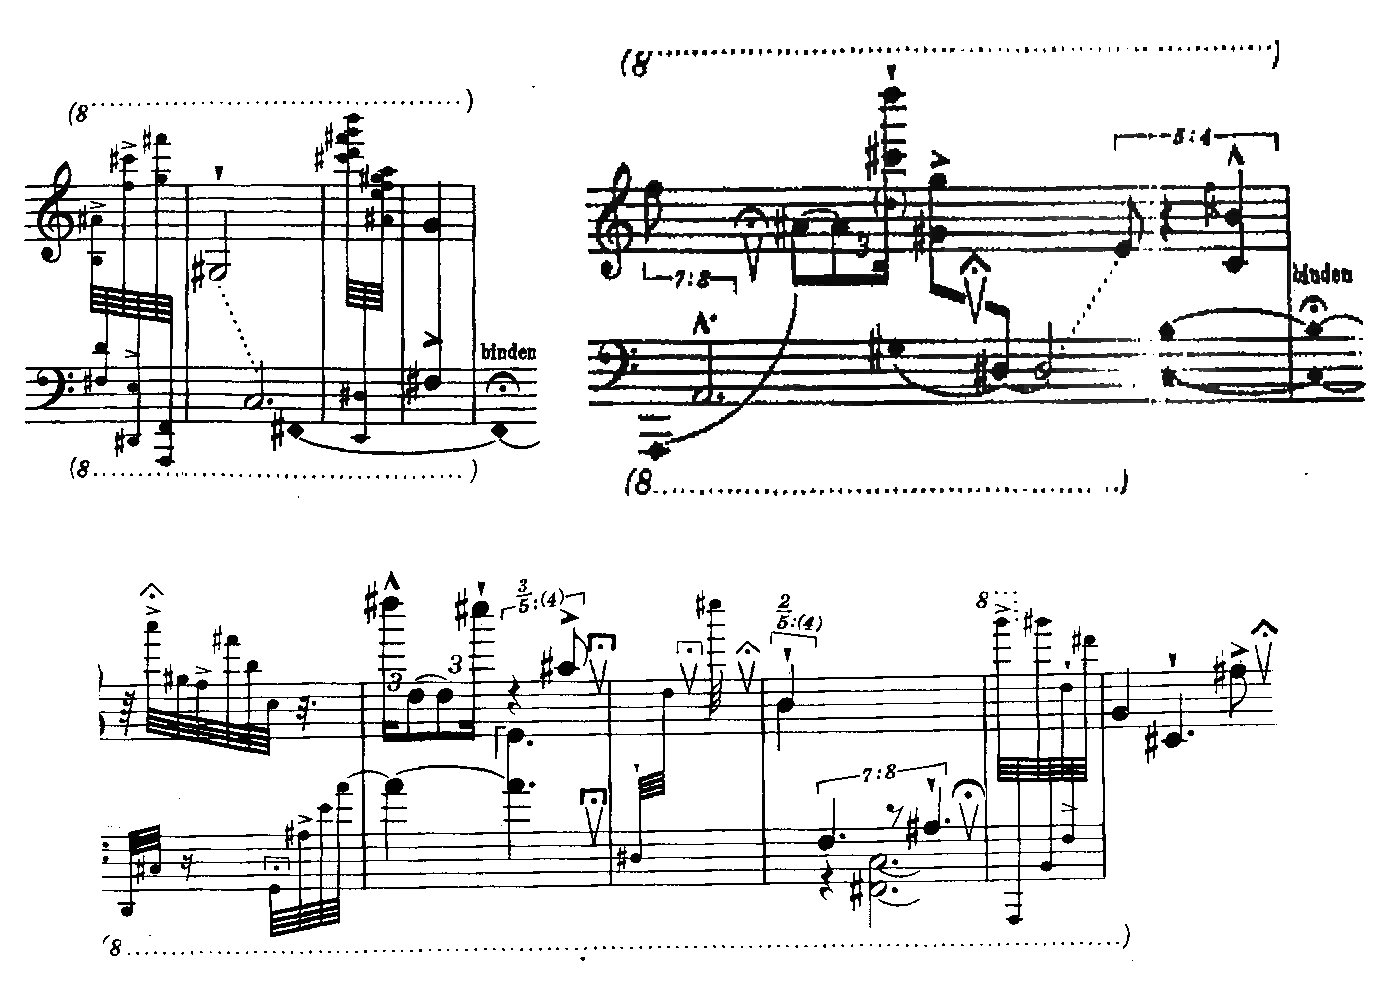
\includegraphics[width=0.9\columnwidth]{klavierstuck.png}
	\caption{Fragments B2, C1, C3 of \klavierstuck{}, Karlheinz Stockhausen.\protect\footnotemark}
	\label{fig.klavierstuck}
	\end{figure}
	\footnotetext{\copyright Copyright 1957 by Universal Edition (London) Ltd., London/UE 12654. Retrieved from \cite{guiguestockhausen}}
	The examples presented in section~\ref{section.examples} allow us to devise the specification for the kind of conditional capabilities that we want to allow composers to express in our notation system.
	Most examples studied here operate at a macroscopic level : the choices of the performer generally concerns sections, but at the phrase level, these are often traditional scores, as can be seen from an excerpt from \klavierstuck{} in fig.~\ref{fig.klavierstuck}. However, the case of a single note which would last longer depending on a given condition can also happen.
	
	The main problem is that there is generally no specific symbol to indicate the conditional execution; instead, the explanation is part of the description of the musical piece. Hence, we have to devise a graphical notation simple enough and yet able to convey easily these different levels of conditions.
	
	These conditions operate on a span of time, which can range from instantaneous, like in the Stockhausen piece, where the performer has to choose his next phrase at the end of the one he is currently playing, to indeterminate, in the case of a perpetual artistic installation waiting for the next visitor. A single symbol might then not be enough to convey in a readable fashion the whole meaning, and multiple symbols would be necessary to explain the articulation of the time in the musical piece.
	
	Finally, an important requirement is to be able to study formal properties on the written score. The presence of conditional expressions means that there is some kind of flow control in the song. Like in a traditional computer software, we want to be able to verify that some properties will remain true for the score : for instance, again in the case of \klavierstuck{}, we would like to be able to specify : \emph{at a given time, there cannot be two overlapping fragments}, and be informed if there might be a possible execution of the score that would lead to this case. This has practical implications especially when working with hardware, which can have hard requirements on the input data. This means that the notation will have to be grounded with solid formal semantics.
	
	\subsection{Formal semantics}\label{section:formalismes}
	The current work is based on previous work at the LaBRI by Jaime Arias, Mauricio Toro and Antoine Allombert, that attempt both to formalize the composition semantics and to provide ways for real-time performance of interactive scores.
	Our work is threefold: finding formal semantics adapted to complex conditional constraints; studying their execution; devising a consistent and simple graphical representation, in order to make the creation of interactive conditional scores as intuitive as possible.
		
	The four following interactive scores formalisms were researched, in order to give a solid foundation, and enforce strong provability properties: 

	\subsubsection{Petri nets}
	One of the most prominent ideas in the research, on which the current implementation of \textsc{i-score} is based, is the use of Petri nets in order to model interactive scores, by focusing on agogic variations.
	
	The followed methodology was to define basic nets for each Allen relationship \cite{allen1983maintaining}, and then to apply a transformation algorithm, described in \cite[section 9.2]{allombert2009aspects}.
	 
	When a score is played, it is compiled by \textsc{i-score 0.2} (shown in fig.~\ref{fig.iscore02}) into a \ac{HTSPN} which is in turn executed using its well-known semantics.
	 
    \begin{figure}[h]
    \centering
    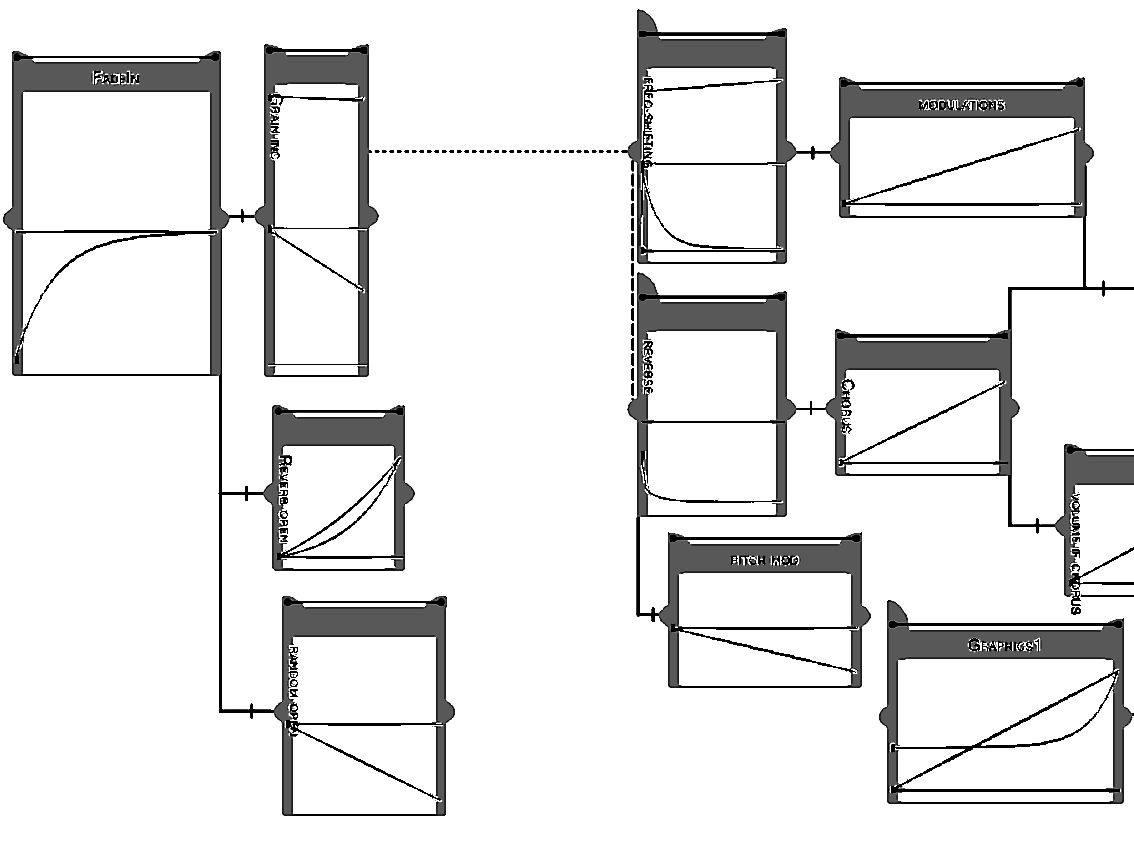
\includegraphics[width=0.9\columnwidth]{iscore-2}
    \caption{i-score 0.2. The model is based on a succession of boxes (containing curves and other boxes), and relationships between these boxes. A box can have trigger points at the beginning and the end; this introduces an unnecessary graphical coupling between the data and the conditions.}
    \label{fig.iscore02}
    \end{figure}
	
	Coloured Petri nets were also used to model complex data processing in interactive scores\cite{arias2014modelling}, in order to allow the description and execution of sound processes to occur directly in the score.
	
	\subsubsection{Temporal Concurrent Constraint Programming} 
	Since the interactive scores can be expressed in terms of constraints ($A$ \emph{is after} $B$), one of the recurrent ideas for their formalisation was to use \ac{NTCC}, since it allows constraint solving. This approach was studied by Antoine Allombert\cite{allombert2006concurrent} and Mauricio Toro\cite{toro2010concurrent, mauricio2012structured}. 
	
	However, there are multiple problems, notably the impossibility to compute easily the duration of a rigid constraint, and the exponential growth of the computation time of constraint solving, which led to some latency in the implementation, making real-time operations impossible.
	
	\subsubsection{Reactive programming}
	Due to the static nature of models involving Petri nets and temporal constraints, a domain-specific language, \textsc{ReactiveIS}\cite{ariasexecuting}, was conceived in order to give dynamic properties to interactive scores. 
	An operational semantic is defined using the synchronous paradigm, to allow both static and dynamic analysis of the interactive scores.
	This also allows composers to easily describe parts of their score that cannot be efficiently represented in a visual manner.

	\subsubsection{Timed Automata}
	The current focus of the research is put upon the investigation of models for the formal semantics of conditional constraints in interactive scores.
	
	This has been achieved using the extendend timed automata of \textsc{UPPAAL}. Timed Automata allow to describe both logical and temporal properties of interactive scores. Moreover, the shared variables provided by \textsc{UPPAAL} allows to model the conditionals.
	They are also used for hardware synthesis, in order to target \acp{FPGA}\cite{arias2015exploiting}. 
	Real-time execution semantics is implemented with this method.
	
	The problem of the implementation of loops is however still unresolved : it makes static analysis on the score harder, since we hurt the reachability problem.
	
	\section{The OSSIA Paradigm}
	\subsection{Presentation}
	OSSIA (Open Scenario System for Interactive Applications) is a research project, presented in \cite{hogue2014ossia} and funded by the french agency for research (ANR).
	Its goal is to devise methods and tools to write and execute interactive scenarios.
	The two main objectives are to provide a formalisation for interactive scenarisation and seamless interoperability with the existing software and hardware.
	This paper will focus on the interactive scoring part, the interoperability being provided by the Jamoma Modular framework \cite{Jamoma-JIM11}, which allows the use of multiple protocols, such as OSC or MIDI.
	% notably by implementing the Minuit\footnote{\href{https://github.com/minuit/minuit}{https://github.com/minuit/minuit}} protocol along with other, more popular protocols such as OSC and MIDI.
	%TODO PB : pê qu'on peut se contenter de dire qu'il implémente plusieurs protocoles... 
	% JM : p-être mettre minuit en footnote? :)
	
	When comparing with the previous approaches for interactive scores (Acousmoscribe, Virage, i-score 0.2), the OSSIA pro\-ject tries to follow a ``users first'' philosophy : the research work is shared and discussed with artists, developers, and scenographers from the musical and theater fields, and their use case serve as a basis for the focus of the research. They are in turn asked to try the software and discuss about the implementation.
	
	For instance, in the previous studies of interactive scores, a mapping had to be done between the theoretical foundation (Petri nets, temporal constraints\dots) and the domain objects with which the composer had to interact.
	This has led to mismatches between the representation and the execution\cite{ariasexecuting} of the score. The most prominent problem was the inability to express cleanly multiple synchronized conditions, and to route the time flow according to these conditions. The formalism also did not allow for boxes directly following each other in a continuous manner, and always required the existence of a relationship between them. 
	Instead, in the OSSIA project, we tried to conceive high-level concepts that would allow a composer to easily write an interactive score, build a software over these concepts, and then implement them on the basis of the formalisms presented in part.~\ref{section:formalismes}.
	
	The main concepts of interactive scores can be grouped in two categories: temporal elements and contents.
	The temporal elements (scenarios, instantaneous events, temporal constraints, conditional branching and hierarchy) allow to create the temporal and logical structure of the scenario, and the contents (states and processes) allow to give actual control over several kind of processes.
	
	\subsection{Temporal elements}
	
\begin{figure}[!t]
	\centering
	\begin{subfigure}[b]{0.9\columnwidth}
		\centering
	    \begin{tikzpicture}
	        \tikzstyle{timenode}=[ultra thick,]
	    	\tikzstyle{constraint}=[ultra thick,]
	    	\tikzstyle{flex}=[very thick,dashed]
    		\tikzstyle{hat}=[ultra thick]
    		\tikzstyle{event}=[circle,thick,fill=black]
	    	\tikzstyle{trigger}=[ultra thick,arrows={-Triangle[angle=45:10pt,fill=white]}]
		
	    	\draw [timenode]   (0, 0) -- (0, 4);
		
			\draw[trigger] (0, 4) -- (0, 3);
	    	\node[event] at (0,3) {};
	    	\node[event] at (0,1) {};
	    \end{tikzpicture}
	    \caption{A Node with two Events, one with a trigger, and one without}
	\end{subfigure}
	
	\begin{subfigure}[b]{0.9\columnwidth}
		\centering
		\begin{tikzpicture}
		\tikzstyle{timenode}=[ultra thick,]
		\tikzstyle{constraint}=[ultra thick,]
		\tikzstyle{flex}=[very thick,dashed]
		\tikzstyle{hat}=[ultra thick]
		\tikzstyle{event}=[circle,thick,fill=black]
		\tikzstyle{trigger}=[ultra thick,arrows={-Triangle[angle=45:10pt,fill=white]}]
		
		
		\node[event] at (0, 0) {};
		\node[event] at (5,0) {};
		\draw[constraint] (0, 0) -- (5,0);
		\end{tikzpicture}
		\caption{A rigid constraint between two events. Minimum and maximum duration of the constraint are equal ; the date of the end event is fixed with regards to the date of the start event.}
	\end{subfigure}
		
	\begin{subfigure}[b]{0.9\columnwidth}
		\centering
	    \begin{tikzpicture}
	        \tikzstyle{timenode}=[ultra thick,]
	    	\tikzstyle{constraint}=[ultra thick,]
	    	\tikzstyle{flex}=[very thick,dashed]
    		\tikzstyle{hat}=[ultra thick]
    		\tikzstyle{event}=[circle,thick,fill=black]
	    	\tikzstyle{trigger}=[ultra thick,arrows={-Triangle[angle=45:10pt,fill=white]}]
		
		
	    	\node[event] at (0, 0) {};
	    	\draw[trigger] (5, 0.01) -- (5, 0);
	    	\node[event] at (5,0) {};
    		\draw[constraint] (0, 0) -- (4,0);
    		\draw[constraint] (4, 0.5) -- (6,0.5);
    		\draw[flex] (4, 0) -- (6, 0);
    		\draw[hat] (4, 0.1) -- (4, 0.5);
	    	\draw[hat] (6, 0.1) -- (6, 0.5);
	    	
	    \end{tikzpicture}
	    \caption{A constraint with a non-null minimum and a different, non-infinite maximum}
	\end{subfigure}
	
	\begin{subfigure}[b]{0.9\columnwidth}
		\centering		
		\begin{tikzpicture}

		\tikzstyle{timenode}=[ultra thick,]
		\tikzstyle{constraint}=[ultra thick,]
		\tikzstyle{flex}=[very thick,dashed]
		\tikzstyle{hat}=[ultra thick]
		\tikzstyle{event}=[circle,thick,fill=black]
		\tikzstyle{trigger}=[ultra thick,arrows={-Triangle[angle=45:10pt,fill=white]}]
		
		\node[event] at (0, 0) {};
		\draw[trigger] (5, 0.01) -- (5, 0);
		\node[event] at (5,0) {};
		
		\draw[constraint] (0, 0) -- (3,0);
		\draw[flex] (3, 0) -- (5,0);
		
		
		\end{tikzpicture}
		\caption{A constraint with a non-null minimum and an infinite maximum}
	\end{subfigure} 
	
	\begin{subfigure}[b]{0.9\columnwidth}
		\centering
		\begin{tikzpicture}
		\tikzstyle{timenode}=[ultra thick,]
		\tikzstyle{constraint}=[ultra thick,]
		\tikzstyle{flex}=[very thick,dashed]
		\tikzstyle{hat}=[ultra thick]
		\tikzstyle{event}=[circle,thick,fill=black]
		\tikzstyle{trigger}=[ultra thick,arrows={-Triangle[angle=45:10pt,fill=white]}]
		
		
		\node[event] at (0, 0) {};
		\node[event] at (5,0) {};
		\draw[flex] (0, 0) -- (5,0);
		\end{tikzpicture}
		\caption{A constraint with a null minimum and an infinite maximum. Instead of making the representation heavier by having the dashes of the constraint continue indefinitely, we chose to remove the rake to symbolize infinity.}
	\end{subfigure}

	\caption{The OSSIA Graphical Formalism}
	\label{fig.graphical}
	\end{figure}
	
	In order to allow the composer to write interactive conditional scores, it is necessary to provide temporal constraints, to allow at least a partial ordering between the different parts of the score. This is done using four base elements : Node, Event, Constraint and Scenario. A \emph{Node} (Time Node) represents a single point in time. An \emph{Event} describes an instantaneous action. A \emph{Constraint} describes the span of time between two given Events.	Finally, the \emph{Scenario} structures the other elements and checks that the temporal constraints are valid and meaningful.

    \subsubsection{Scenario}
    A Scenario is defined as an union of directed acyclic graphs. The vertices are Events and the edges are Constraints. The direction is the flow of time. It allows to organize the other base elements in time. 
    
	Scenarios follow these basic rules:
	\begin{itemize}
		\item A Scenario begins with a Node
		\item There can be multiple Events explicitly synchronized by a single Node
		\item A Constraint is always started by an Event and finished by another, distinct Event
	\end{itemize}
	
	Events and Constraints are chained sequentially. Multiple Constraints can span from a single Event and finish on a single Event, as shown in fig.~\ref{fig.timeNode}. The operational semantics of these cases will be described later. This allows different processes to start and/or stop in a synchronized manner.

	\subsubsection{Events and Nodes}\label{section.events}
	An Event allows to describe precisely a part of what will happen in a specific, instantaneous point in the execution of the score.
	It is the basic element, to which are further attached Constraints.
	
	Events can be explicitly synchronized using Nodes.
    This means that when an Event is triggered, all the other Events on the same Node are also evaluated and instantaneously triggered (or discarded if their Condition is not met, see section~\ref{Conditions}).
    
	\subsubsection{Constraints}
	A Constraint represents a span of time. Due to the interactive nature of the proposed paradigm, the span can change at execution time, like a \textit{fermata}. When the author wants to allow a Constraint to have a variable duration, he renders it flexible. This means that the end of the Constraint depends on the Condition of its final Event.
	
	A Constraint can be activated or deactivated: if it is deactivated, it will not count for the determination of the execution span of its end event.
	
	The graphical representation of a Constraint can change according to its minimum and maximum duration. The minimum $m$'s range is $[0; +\infty]$, and the maximum $M$'s range is $[m; +\infty] \setminus{\{0\}}$. In the user interface (introduced in section~\ref{section.userinterface}), the duration is directly linked to the horizontal size and is visible on a ruler.
	
	\subsubsection{Graphical formalism}
	The graphical formalism for these elements is presented in fig.~\ref{fig.graphical}.
	
	The Node is a vertical line. 
	An Event is a dot on a Node. 
	If there is a trigger on the Event, a small arrow indicates it. The colour of the arrow can change at run-time to indicate the current state of the trigger.
	
	The Constraint is an horizontal line that represents a span of time, like a timeline. If the constraint is flexible, the flexible part is indicated by dashes and a rake. When there is no maximum to the constraint, there is no rake.
	\subsection{Operational semantics}
	
	\begin{figure}
	\centering
	%\resizebox{0.9\columnwidth}{!}{
		\begin{tikzpicture}[scale=0.5]	
		\tikzstyle{timenode}=[ultra thick,]
		\tikzstyle{constraint}=[ultra thick,]
		\tikzstyle{flex}=[very thick,dashed]
		\tikzstyle{hat}=[ultra thick]
		\tikzstyle{event}=[circle,thick,fill=black]
		\tikzstyle{trigger}=[ultra thick,arrows={-Triangle[angle=45:10pt,fill=white]}]
		
		\draw [timenode]   (9, 0) -- (9, 6);
		
		\node[event, label=A] at (5,5) {};
		\node[event, label={[label distance=1.5mm]55:B}] at (9,5) {};
		\draw [constraint] (5, 5) -- (9, 5);
		
		
		\draw [trigger] (9, 3.1) -- (9,3);
		\node[event, label={[label distance=1.5mm]55:C($/x = 1$)}] at (9,3) {};
		\node[event, label=D] at (14,3) {};
		\draw [constraint] (9, 3) -- (14, 3);
		
		
		\draw [trigger] (9, 1.1) -- (9, 1);
		\node[event, label={[label distance=1.5mm]55:E($/x \neq 1$)}] at (9,1) {};
		\node[event, label=F] at (14,1) {};
		\draw [constraint] (9, 1) -- (14, 1);
		\end{tikzpicture}
	%	}
	\caption{Implementation of temporal branching. $A, B, C, D, E, F$ are Events. $B, C, E$ are on the same Node. $C$ contains the condition $/x = 1$ and $E$ contains $!(/x = 1)$ in order to have an \emph{if - then - else} mechanism. $C$ and $E$ are evaluated when the constraint between $A$ and $B$ has ended.}
	\label{fig.ifelse}
	\end{figure}
	
	\begin{figure}
	\resizebox{0.9\columnwidth}{!}{
	\begin{tikzpicture}[scale=0.5]	
		\tikzstyle{timenode}=[ultra thick,]
		\tikzstyle{constraint}=[ultra thick,]
		\tikzstyle{flex}=[very thick,dashed]
		\tikzstyle{hat}=[ultra thick]
		\tikzstyle{event}=[circle,thick,fill=black]
		\tikzstyle{trigger}=[ultra thick,arrows={-Triangle[angle=45:10pt,fill=white]}]
		
		% Premier timenode (B)
		\draw [timenode]   (9, 0) -- (9, 12);
		
		\node[event, label=A] at (7,11) {};
		\node[event, label={[label distance=1mm]55:B}] at (9,11) {};
		\draw [constraint] (7, 11) -- (9, 11);
		
		\node[event, label={[label distance=1mm]55:C($/x = 1$)}] at (9,9) {};
		\node[event, label={[label distance=1mm]55:D}] at (18,9) {};
		\draw [constraint,dashed] (9,9) -- (18,9);
		
		\node[event, label={[label distance=1mm]55:E($/x \neq 1$)}] at (9,1) {};
		
		\node[event, label={[label distance=1mm]55:F}] at (14,1) {};
		\draw [constraint,dashed] (9, 1) -- (14, 1);
		
		
		% Second timenode (D)
		\draw [timenode]   (18, 4) -- (18, 10);
		\node[event, label={[label distance=1mm]55:G($/y = 1$)}] at (18,7) {};
		\node[event, label=H] at (22.2,7) {};
		\draw [constraint] (18,7) -- (22.2,7);
		
		
		\node[event, label={[label distance=1mm]55:I($/y \neq 1$)}] at (18,5) {};
		\node[event, label=J] at (22,5) {};
		\draw [constraint] (18,5) -- (22,5);
		
		
		% Troisieme timenode (F)
		\draw [timenode]   (14, -6) -- (14, 2);
		
		
		\node[event, label={[label distance=1mm]55:K($/z = 1$)}] at (14,-2) {};
		\node[event, label=L] at (20,-2) {};
		\draw [constraint] (14,-2) -- (20,-2);
		
		
		\node[event, label={[label distance=1mm]55:M($/z \neq 1$)}] at (14,-5) {};
		\node[event, label=N] at (19,-5) {};
		\draw [constraint] (14,-5) -- (19,-5);
		
		
		\draw [trigger] (9, 9.1) -- (9, 9);
		\draw [trigger] (9, 1.1) -- (9, 1);
		\draw [trigger] (18, 7.2) -- (18,7);
		\draw [trigger] (18, 5.1) -- (18,5);
		\draw [trigger] (14, -1.9) -- (14,-2);
		\draw [trigger] (14, -4.9) -- (14,-5);
		\end{tikzpicture}
		}
	\caption{Nested \emph{if - then - else} using flexible constraints}
	\label{fig.nestedifelse}
	\end{figure}
	
	\subsubsection{Conditions}\label{Conditions}
	Each Event carries a condition of execution, and a maximum range of time for its evaluation.
	The effective range of time for execution is computed by constraint-solving algorithms. 
	For the Event to enter its execution range, all the Constraints that finish on this Event must be between their minimal and maximal duration. 
	
	An Event is executed as soon as its condition evaluates to True in its execution range. As a result, the Constraints that follow this Event are started, and the messages that might be stored in the Event are sent.
	Otherwise, the Event is discarded and all the following Constraints are deactivated.
	
	There is usually a default condition which is ``all the constraints that explicitly finish on the event have ended''.
	This default condition can be replaced or extended.
	For instance, there can be checks on the arrival of a specific network message, or checks on a remote or local address's value with a specific expression, with the following syntax:
	\begin{itemize}
	\item For parameters that can have a value, there can be comparisons between the values. For instance:
	\begin{lstlisting}[breaklines]
/some/parameter > 35 && 
(   /other/parameter != "a string" 
 || /last/parameter == true)
    \end{lstlisting}
	\item Value-less parameters (akin to \emph{bangs} in PureData) can also be used as triggers for the evaluation of expressions. In this mode, logical operators have a different meaning. For instance: \\ \texttt{/some/bang \&\& !/another/bang} \\ will trigger if : 
	\begin {itemize}
	    \item \texttt{/some/bang} is received, and 
	    \item \texttt{/another/bang} is not received within the synchronization interval. 
	\end{itemize}
	\item This is not to be confused with the comparison with boolean values : 
	\begin{lstlisting}[breaklines]
/a/val == true && 
/another/val == false
    \end{lstlisting} which will trigger when the parameters will both be set (not necessarily at the same time) to the required values.
	
	\end{itemize}
	
	Higher-level operations, like a mouse click on a GUI can then be translated in conditions on Events, in order to bring rich interaction capabilities to the software dedicated to the execution of the scores.
	
	\subsubsection{Conditional branching}
	Branching occurs when, at a single point in the score, two different executions can happen, which leads the scenario to distinct states.
	For example, the classic \emph{if - then - else} construct can be implemented by having two Events with opposite conditions, as shown in fig.~\ref{fig.ifelse}.
	It is also possible to have other cases : for instance, there could be a set of conditions that would lead to either both constraint, or no constraint executed. It is also possible to have multiple constraints with the same condition.
	Figure~\ref{fig.nestedifelse} presents a method to instantaneously nest conditions, using a flexible constraint with a minimal duration of zero. 
	These patterns can be used as is. 
	However, the authoring software should provide graphical ways to simplify these common cases, for instance by not showing the duplicated conditions. This is not yet done in the current development version of i-score, which allows its users to author scores using the raw formalism presented here.
	
	Convergence occurs when we want to synchronize parts of a scenario that branched previously. The constraint solver ensures that the durations are coherent during the authoring of the score. The execution date of the Node for which a convergence happens will necessarily be after the minimum of each converging Constraint.
	
	\subsubsection{Execution of a Node}
	In this part, we will first present a high-level algorithm that explains the general order of execution of a Node. Then, we will study a particular Node and see how the algorithm translates into a Petri net that can be executed for this particular Node.
	
	As we said before in section~\ref{section.events}, Events are attached to a Node. They are ordered  and will be evaluated one after another according to the algorithm given in fig.~\ref{fig.algTimeNode}. 
	\begin{figure}[h]
		\begin{algorithmic}
			\Require{We enter the evaluation range for a Node $n$}
			
			\If{all($n$.eventList(), Event::emptyCondition)}
			\Repeat
			\State{wait()}
			\Until{$n$.DefaultDate}
			\For {Event $e$ in $n$.eventList()}
			\State{$e$.run()}
			\EndFor
			\Else
			\Repeat
			\If{any($n$.eventList(), Event::isReady)}
			\State{nodeWasRun $\leftarrow$ true}
			\For {Event $e$ in TimeNode.eventList()}
			\If {validate($e$.condition())}
			\State{$e$.run()}
			\Else
			\State {$e$.disable()}
			\EndIf
			\EndFor
			\EndIf       
			
			\Until{nodeWasRun}
			\EndIf
		\end{algorithmic}
	
	\caption{Execution algorithm for a Node}
	\label{fig.algTimeNode}
	\end{figure}
	
	The software guarantees that at a high level, if the composer sets an order, the messages will be sent in this order. The only delay will be the one induced by the ordering of instructions in the CPU.
	
	However, it is necessary to be aware that the protocols used underneath, like UDP which is commonly used in OSC protocol implementations, might not always have such strong guarantees.
	For this reason, and also because it is not possible to expect network messages to arrive exactly at the same time, the author can specify a synchronization time on a Node: it can wait for a brief time after the triggering of another Event in the same Node, in order to let some time for messages to be received and change the result of conditional choices. However we don't have yet a way to represent this graphically; the idea of a bolder time node was proposed.
	The synchronization time can also express the will to synchronize events at a lower rate, like two people clapping hands at the same time for example.
	
	Another possibility for the ordering would be to run the Event whose condition did trigger the time node first, and then run the others. This should be a choice left at the discretion of the score writer.
	
	Figure~\ref{fig.timeNode} presents the different branching and converging cases that may occur, all mixed in a single Node. 
	
	\begin{figure}[h]
	\resizebox{0.9\columnwidth}{!}{
		\tikzset{>=latex}
		\begin{tikzpicture}[scale=0.4]
		\tikzstyle{timenode}=[ultra thick,]
		\tikzstyle{constraint}=[ultra thick,]
		\tikzstyle{flex}=[very thick,dashed]
		\tikzstyle{hat}=[ultra thick]
		\tikzstyle{event}=[circle,thick,fill=black]
		\tikzstyle{trigger}=[ultra thick,arrows={-Triangle[angle=45:10pt,fill=white]}]
		
		\draw [timenode]   (9, 0) -- (9, 14);
		
		\node[event, label=A] at (2,12) {};
		\node[event, label={[label distance=1.5mm]55:B}] at (9,12) {};
		\draw [constraint] (2, 12) -- (6, 12);
		\draw [constraint] (6, 12.7) -- (12, 12.7);
		\draw [flex] (6, 12) -- (12, 12);
		\draw [hat] (6, 12.1) -- (6, 12.7);
		\draw [hat] (12, 12.1) -- (12, 12.7);
		\draw [trigger] (9, 13) -- (9, 12);
		
		\node[event, label=C] at (0,10) {};
		\draw [constraint] (0, 10) -- (6, 10);
		\draw [constraint] (6, 10.7) -- (12, 10.7);
		\draw [flex] (6, 10) -- (12, 10);
		\draw [hat] (6, 10.1) -- (6, 10.7);
		\draw [hat] (12, 10.1) -- (12, 10.7);
		
		
		\node[event, label=D] at (15,8) {};
		\draw [constraint] (9, 8) -- (15, 8);
		
		\node[event, label=E] at (3,5) {};
		\draw [trigger] (9, 6) -- (9, 5);
		\node[event, label={[label distance=1.5mm]55:F}] at (9, 5) {};
		
		\draw [constraint] (3, 5) -- (6, 5);
		\draw [constraint] (6, 5.7) -- (12, 5.7);
		\draw [flex] (6, 5) -- (12, 5);
		\draw [hat] (6, 5.1) -- (6, 5.7);
		\draw [hat] (12, 5.1) -- (12, 5.7);
		
		\node[event, label={[label distance=1.5mm]55:G}] at (9,3) {};
		\node[event, label=H] at (14, 3) {};
		\draw [constraint] (9, 3) -- (14, 3);
		
		\node[event, label=I] at (16, 1) {};
		\draw [constraint] (9, 1) -- (16, 1);
		\end{tikzpicture}
		}
		\caption{A complete example of Node in the OSSIA graphical formalism. Two constraints converge on the Event $B$, and three constraints branch from the Node that synchronizes $B, F, G$. The durations are already processed by the constraint solver.}
		\label{fig.timeNode}
	\end{figure}
	
	\subsection{Contents}
    An Event may contain a State, which contains messages, and can itself hierarchically contain other States. 
	At a conceptual level, for the composer, a State generally represents a change of state in a remote or local device, i.e.~a discontinuity.
	
	A Constraint also acts as a container: during its execution, several Processes can be executed in parallel.
	
	The two main Processes are:
	\begin{itemize}
		\item The Curve, which allows to send interpolated data in any protocol available to the software.
		%JMCo : est-ce qu'on ne pourrait pas remplacer The Curve par Data process ou qqc du genre ? 
		\item The Scenario, which allows hierarchy to happen seamlessly: a constraint can contain a scenario, which can in turn contain other Constraints.
	\end{itemize}
	
	There can be two possible executions for processes: they can do something on each tick of a scheduler; or they can send start and stop signals and behave however they want in-between.
	
	Processes can share data with the Events at the beginning and the end of the parent Constraint, by putting them in specific States. 
	
	The API provides ways for somebody to implement his own processes and use them afterwards in scores.

	
	\begin{figure}
	\centering
	\resizebox{0.9\columnwidth}{!}{
\begin{tikzpicture}[font=\footnotesize,auto]
\tikzstyle{arc}=[->,>=stealth,thick]
\tikzstyle{place}=[circle,thick,minimum size=6mm,draw=black!75]
\tikzstyle{every transition} = [fill=black,minimum width=1.5mm,minimum height=5mm]
\tikzstyle{every token}=[fill=black,text=black]
%% TikZ-figure elements %%
\node[place,label=$\mathrm{Cond_B}$] at (1.6,-0.3) (P0) {};
\node[place,] at (1.6,-1.4) (P1) {};
\node[place,] at (1.6,-2.5) (P2) {};
\node[place,tokens=1] at (1.6,-3.5) (P3) {};
\node[place,] at (5.7,-1.9) (P4) {};
\node[place,] at (9.3,-2.7) (P5) {};
\node[place,] at (11.5,-2.7) (P6) {};
\node[place,] at (6.8,-4.4) (P7) {};
\node[place,] at (4.6,-5.2) (P8) {};
\node[place,tokens=1] at (5.2,-6) (P9) {};
\node[place,] at (6.8,-6.0) (P10) {};
\node[place,label=$\mathrm{Cond_F}$] at (1.6,-5.2) (P11) {};
\node[place,] at (1.6,-6.3) (P12) {};
\node[place,tokens=1] at (1.6,-7.4) (P13) {};
\node[place,] at (9.3,-6.8) (P14) {};
\node[place,] at (11.5,-6.3) (P15) {};
\node[place,] at (11.5,-7.4) (P16) {};
\node[transition,label=$\mathrm{AB_{min}}$] at (0.5,-1.4) (T0) {};
\node[transition,label=$\mathrm{CB_{min}}$] at (0.5,-2.5) (T1) {};
\node[transition,] at (3.5,-1.9) (T2) {};
\node[transition,] at (8.2,-1.9) (T3) {};
\node[transition,label=$\mathrm{Passive}$] at (8.2,-3.5) (T4) {};
\node[transition,] at (10.6,-2.7) (T5) {};
\node[transition,label=$\mathrm{BD_{min}}$] at (12.5,-2.7) (T6) {};
\node[transition,label=$\mathrm{T_{sync}}$] at (6.0,-5.2) (T7) {};
\node[transition,label=$\mathrm{EF_{min}}$] at (0.4,-6.3) (T8) {};
\node[transition,] at (3.4,-6.3) (T9) {};
\node[transition,] at (8.2,-6.8) (T10) {};
\node[transition,] at (10.6,-6.8) (T11) {};
\node[transition,label=$\mathrm{GH_{min}}$] at (12.5,-6.3) (T12) {};
\node[transition,label=$\mathrm{GI_{min}}$] at (12.5,-7.4) (T13) {};
\node[transition] at (8.2,-7.8) (T14) {};
\draw[arc] (T0) to[bend right=0]  (P1) {};
\draw[arc] (T1) to[bend right=0]  (P2) {};
\draw[arc] (P0) to[bend right=0] node[midway,auto] {} (T2) {};
\draw[arc] (P1) to[bend right=0] node[midway,auto] {} (T2) {};
\draw[arc] (P2) to[bend right=0] node[midway,auto] {} (T2) {};
\draw[arc] (P3) to[bend right=0] node[midway,auto] {} (T2) {};
\draw[arc] (T2) to[bend right=0]  (P4) {};
\draw[arc] (P4) to[bend right=0] node[midway,auto] {} (T3) {};
\draw[arc] (T3) to[bend right=0]  (P5) {};
\draw[arc] (P5) to[bend right=0] node[midway,auto] {} (T5) {};
\draw[arc] (T5) to[bend right=0]  (P6) {};
\draw[arc] (P6) to[bend right=0] node[midway,auto] {} (T6) {};
\draw[arc] (T4) to[bend right=0]  (P5) {};
\draw[arc] (P7) to[bend right=0] node[midway,auto] {} (T4) {};
\draw[arc] (P7) to[bend right=0] node[midway,auto] {} (T3) {};
\draw[arc] (T7) to[bend right=0]  (P7) {};
\draw[arc] (P8) to[bend right=0] node[midway,auto] {} (T7) {};
\draw[arc] (P9) to[bend right=0] node[midway,auto] {} (T7) {};
\draw[arc] (T7) to[bend right=0]  (P10) {};
\draw[arc] (T8) to[bend right=0]  (P12) {};
\draw[arc] (P11) to[bend right=0] node[midway,auto] {} (T9) {};
\draw[arc] (P12) to[bend right=0] node[midway,auto] {} (T9) {};
\draw[arc] (P13) to[bend right=0] node[midway,auto] {} (T9) {};
\draw[arc] (P3) to[bend right=0] node[midway,auto] {} (T4) {};
\draw[arc] (P10) to[bend right=0] node[midway,auto] {} (T10) {};
\draw[arc] (T10) to[bend right=0]  (P14) {};
\draw[arc] (P14) to[bend right=0] node[midway,auto] {} (T11) {};
\draw[arc] (T11) to[bend right=0]  (P15) {};
\draw[arc] (P15) to[bend right=0] node[midway,auto] {} (T12) {};
\draw[arc] (T11) to[bend right=0]  (P16) {};
\draw[arc] (P16) to[bend right=0] node[midway,auto] {} (T13) {};
\draw[arc] (T9) to[bend right=0]  (P8) {};
\draw[arc] (T2) to[bend right=0]  (P8) {};
\draw[arc] (P13) to[bend right=0] node[midway,auto] {} (T14) {};
\draw[arc] (P7) to[bend right=0] node[midway,auto] {} (T14) {};
\end{tikzpicture}
}
	\caption{Petri net for the Node of fig.~\ref{fig.timeNode}.\\*
	The previous Constraints's minimum duration have to elapse in $\mathrm{AB_{min}}$, $\mathrm{CB_{min}}$, $\mathrm{EF_{min}}$. When a Condition is validated, a token is put in the respective place ($\mathrm{Cond_B}$ or $\mathrm{Cond_F}$); this triggers the evaluation of the whole Node, unless it was already triggered. The central transition $\mathrm{T_{sync}}$ introduces a small synchronization delay to allow other conditions to validate if necessary. When an Event's condition is not validated, a passive token is instead sent to the following Constraints, which will not trigger the execution of any process or state, and will simply allow the scenario to keep going after a failed condition.
	This is achieved by the $\mathrm{Passive}$ transition.}
	\label{fig.petri}
	\end{figure}
	
	\subsection{Usage as an API}\label{section.api}
	One of the goals of this high-level paradigm is to allow at the same time, a simple mapping with graphical elements, clear semantics of execution, and simple translations with the proven semantics that were studied before, like Petri nets and Timed Automata. In this way, a composer could describe his score which could then be translated into a variety of formats that allow for static and dynamic analysis.
	
	This is achieved by writing a C++ API, that allows for multiple implementations and the use generic programming. It is accessible in \url{https://github.com/OSSIA/API}. It consitutes a kind of domain-specific language, with the elements that were talked about earlier.
%	An example of usage is shown in Figure~\ref{fig.api}.
%	
%	\begin{figure}[h]
%		\begin{lstlisting}
%Device<OSC> player{"127.0.0.1:1234",
%                   "player"};
%Device<Minuit> video{"127.0.0.1:1235",
%                     "video"};
%Scenario s;
%CurveProcess curve{
%        player.addr("volume"), 
%        {{0.0, 0.0}, 
%        {0.5, 0.8}, 
%        {1.0, 0.0}}};
%Constraint c1;
%c1.setDuration(2_s);
%c1.addProcess(curve);
%State s1{player.addr("start")};
%State s2{player.addr("stop"),
%         video.addr("flash", 
%                    255, 255, 255)};
%Event e1, e2;
%e1.addState(s1);
%e2.addState(s2);
%Node n1 = s.getStartNode();
%n1.addEvent(e1);
%Node n2;
%n2.addEvent(e2);
%s.addConstraint(c1, n1, n2);
%s.play();
%		\end{lstlisting}
%		\caption{Example of usage of the OSSIA API}
%		\label{fig.api}
%	\end{figure}
%	
	% \subsection{Comparison}
	% Pour une éttude formelle de l'API
	% - http://dl.acm.org/citation.cfm?id=1248863
	% - http://itu.dk/stud/speciale/gamelib/APIUsability.pdf
	% - http://ieeexplore.ieee.org/xpl/login.jsp?tp=&arnumber=4639083&url=http%3A%2F%2Fieeexplore.ieee.org%2Fxpls%2Fabs_all.jsp%3Farnumber%3D4639083
	% - http://dl.acm.org/citation.cfm?id=1718957
	
	
	\subsection{Implementation in terms of Petri nets}
	In order to maintain cohesiveness with the previous works on the field, we chose to represent the temporal logic of our formalism in terms of Petri nets. The span of time of the constraints is represented as a transition, and states are emitted when a token enters a state-containing place. These places are not represented here because there can be multiple cases according to the requirements of the writer of the score: it would for instance be possible to send the last state either after the default duration of the constraint, or as soon or late as the condition is validated.
	It is also possible to add places and transitions in order to have a specific behaviour occurs when the maximum duration of a constraint elapses without triggering.
	
	Figure~\ref{fig.petri} represents the translation of the Node shown in fig.~\ref{fig.timeNode} into Petri nets. We refer to Constraints by the name of their start and end Events. 

	\section{i-score: Temporal and Logical user interfaces}
	\label{section.userinterface}
	\begin{figure}
	\centering
	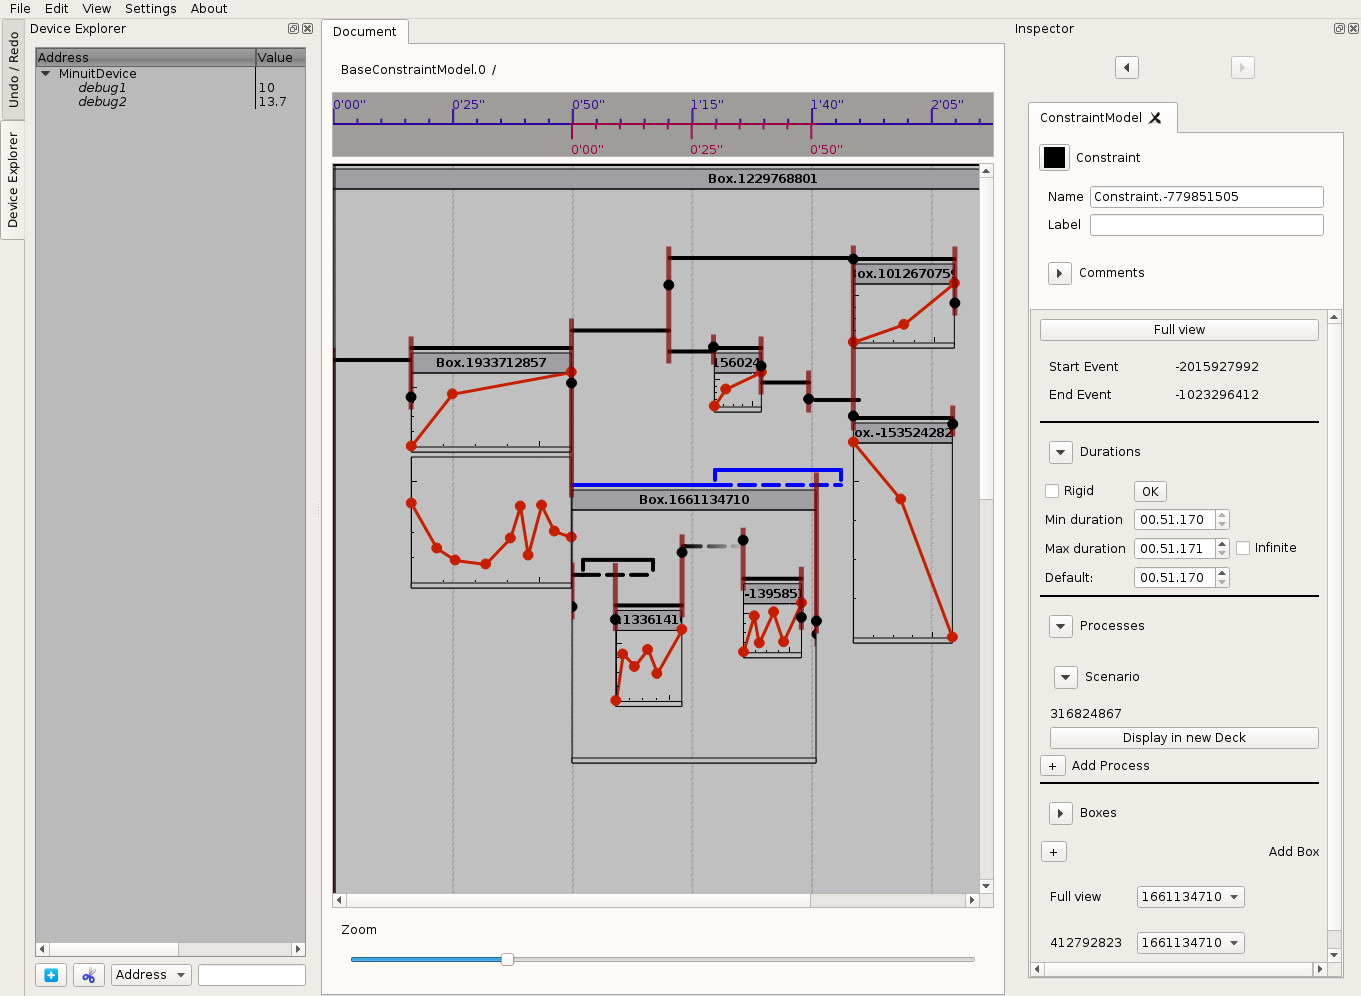
\includegraphics[width=0.9\columnwidth]{iscoreArticle.png}
	\caption{An example of score in i-score 0.3. Not all the graphical features presented here are already implemented.}
	\label{fig.iscore03}
	\end{figure}
	
	The API talked about in section~\ref{section.api} is being used as the basis of different projects tied to the interactive scores. The dependency graph is shown in fig.~\ref{fig.softwares}.

	The different sub-projects are: 
	\begin{itemize}
	\item \textsc{i-score}, a graphical editor and player for the interactive scores. It solves the problem of the display, edition and interaction with simultaneous elements of the interactive scores. Its current development version (0.3) is available at  (\url{https://github.com/OSSIA/i-score}).
	\item \textsc{j.score} and \textsc{i-score-cmd}: two players for the scores produced in i-score. The first is an external for Max, the second is a standalone command-line executable. Their current version is available in the repository of the Jamoma project (\url{https://github.com/Jamoma/Jamoma}).
	\end{itemize}

    \textsc{i-score} also exposes its own dynamic device in order to provide some kind of external control at run-time. For example, the conditions could be changed prior to their evaluation, in order to set them in advance at true or false according to events that might have occurred previously during the execution of the score. 
    
    The current version (0.2) of \textsc{i-score}, shown in fig.~\ref{fig.iscore02}, relies on the idea that relations are used to separate boxes. At the time of writing, the upcoming version (0.3, shown in fig.~\ref{fig.iscore03}) is able to create constraints, events, and nodes using the graphical formalism that was presented in this article, and can play and export these scores so that they can be played on the other software of the suite.
    It also allows a primitive form of collaborative edition of scores on a local network, and the authoring and execution of distributed scores is currently being studied. Distributed scores would allow for instance to have a part of a score run on a computer, and another part run on another computer.
    
	\begin{figure}[h]
	\resizebox{0.9\columnwidth}{!}{
		\begin{tikzpicture}[node distance=1cm, auto]
		\node[box] (api) {OSSIA API};
		\node[box,below=0.5cm of api] (impl) {JamomaScore}; 
		\node[box,above left=0.4cm of api] (toolkit) {API toolkit};
		
		\node[box,below=0.4cm of toolkit] (zerotwo) {i-score 0.2};
		\node[box,above=0.4cm of toolkit] (iscore) {i-score 0.3};
		\node[box,above=of api] (cmd) {i-score-cmd};
		\node[box,right=0.8cm of cmd] (jscore) {j.score};
		
		\node[box, right=0.8cm of api] (formats) {Translations formats};
		
		\draw[link] (impl) -- (api);
		\draw[link] (api) -- (toolkit);
		\draw[link] (toolkit) -- (iscore);
		\draw[link] (api) -- (cmd);
		\draw[link] (api) -- (jscore);
		\draw[link] (api) -- (formats);
		\draw[link] (formats) -- (api);
		\draw[link] (impl) -- (zerotwo);
		\end{tikzpicture}
	}
		\caption{Diagram of the different components of the OSSIA project}
		\label{fig.softwares}
	\end{figure}	
\section{Conclusion}
	We presented in this article a new interactive score semantic that allows the conception and execution of conditional scores. This semantic is thought of as a mapping into well-known formal models, such as Petri nets, Timed Automata, and Reactive languages: it is meant to be easily understandable and usable for the composer.
	
	However, in order to achieve more expressive power, we still need to find a way to implement loops. Two approaches are currently being studied: one using a Loop process, and another using a concept of \texttt{goto}; once one is chosen, we will try to find a relevant graphical element to present it.
	
	Furthermore, there could be some interest in the specification and implementation of variables, which could alleviate the need for an adjacent software like Max/MSP to perform complex logical computations. This would maybe pave the way towards a time-oriented Turing complete programming language, with a simple graphical representation which would allow composers to write complex scores in an understandable way.
	Another track is the implementation of an audio engine, for instance by embedding FaUST\footnote{\url{http://faust.grame.fr/}}, in order to be able to produce sound directly from i-score. The relevant parameters would then be exposed and controlled within i-score.
	
	The next step for the graphical formalism is to make usability studies in order to find the most convincing interactions in the authoring software for the composers.
	
	\subsection*{Acknowledgements}
	The authors would like to thank Théo~de~la~Hogue as well as Jaime~Arias for their contributions and insightful comments during the writing of this article. The OSSIA project was funded by the french agency for research (ANR) under the reference ANR-12-CORD-0024 for the 2012-2015 period.
	
	\bibliographystyle{alpha}
	\bibliography{ossia_tenor2015}
\end{document}